\chapter{Implementación}

\noindent\fbox{
	\parbox{\textwidth}{
		Tras lo previsto en el anterior capítulo, aquí se comentará cómo se ha realizado el sistema resultante, en base a la planificación y los diseños, de forma que se acabe con, al menos, un Producto Mínimo Viable.
	}
}
\newline

La implementación del software se ha dividido en los anteriores sprints. Estos, han sido definidos anteriormente en el Backlog, al que iremos haciendo referencia durante los sprints.

Además, para ir guardando el progreso y controlar los cambios, se ha optado por usar el sistema de versiones Git y utilizar a GitHub como forja en la nube, ya que al estar en Internet se puede acceder al proyecto en cualquier dispositivo. En este caso, el repositorio está alojado \href{https://github.com/IvanitiX/TFG\_AsistenteVozModular}{en este enlace} 

También se ha tratado de hacer varias pruebas teniendo de base los ejemplos establecidos en los Casos de Uso discutidos en el epígrafe \ref{casos-uso}. Si bien puede que no se acaben haciendo esas funciones, necesitaremos ver cómo se comportan para poder evaluar lo que podemos hacer con el sistema.

\section{Sprint 1}
En este primer sprint, nuestro objetivo principal es poder interactuar con el ordenador usando la voz, lo que implica hacer que reproduzca sonidos y nos escuche usando el hardware disponible, así como conseguir que este nos pueda reconocer qué estamos diciendo y que si le entregamos un texto nos lo pueda leer .

Dicho esto, este sería el Sprint Backlog:
\begin{table}[H]
	\begin{tabularx}{\textwidth}{|c|X|}
		\hline
		{\cellcolor{mintgreen}} \textbf{Nº ID} & {\cellcolor{mintgreen}} \textbf{Descripción} \\
		\hline
		1 & RF-1. Hablar al Asistente \\
		\hline
		2 & RF-2. Escuchar una respuesta del Asistente \\
		\hline
		3 & RF-3. Sintetizar la voz de una pregunta en un texto \\
		\hline
		4 & RF-4. Generar un audio leyendo una respuesta \\
		\hline
	\end{tabularx}
\end{table}

\subsection{Implementación de la reproducción de audio}
Para esta parte se hizo un adaptador genérico con el único método que necesitaríamos
de los reproductores: Reproducir un archivo con el método \texttt{play()}

Tras ello se implementaron dos versiones del reproductor con base en ese adaptador,
usando PyAudio \cite{pyaudio} y FFMpeg \cite{ffmpeg}. En ambas plataformas se pudo implementar fácilmente, aunque PyAudio es más sencillo de integrar pero enfocado en archivos \texttt{.wav}, mientras que para usar FFMpeg había que usar el comando \texttt{ffplay} con las opciones, aunque este nos permite usar cualquier archivo de audio, incluso streamings de audio, como puede ser la radio por Internet.

\subsection{Implementación de la grabación de audio}
Para esta parte se hizo un adaptador genérico con el método que necesitaríamos
de los reproductores: Reproducir un archivo con el método \\ \texttt{record\_audio()}. De cara al futuro, también deberíamos permitir encauzar los datos que salen del micrófono para tratarlos posteriormente con el método \texttt{stream\_audio()}

En este caso se ha querido realizar algo similar con respecto al punto anterior, pero la grabación del audio desde FFMpeg daba una señal con muchas interferencias, debido a que se debe apuntar a una interfaz hardware concreta, a diferencia de PyAudio, que usa el dispositivo por defecto. Así, al coger el audio del micrófono interno, se generaba mucho ruido de lo que captaba alrededor de este.

\subsection{Adaptación de la API de Speech Recognition}
Tal como se discutió en el anterior capítulo, se acabó eligiendo Vosk\cite{vosk}, el cual tiene una librería en Python a través de pip que nos permitía usarla.
Para permitir el desarrollo de futuros adaptadores para otros sistemas de Reconocimiento del Habla, se ha optado por hacer otra Interfaz que sirva de marco para definir los métodos que se usarán en nuestro sistema.
De esta interfaz se implementará la clase \texttt{VoskAdapter} del cual podemos sacar la transcripción de un audio.

\subsection{Implementación del streaming de audio}
A la hora de hacer las pruebas surgía una inquietud. Habría que perder un tiempo en grabar y pasarlo al sistema de reconocimiento del habla, de un audio que luego se borraría y puede ocupar espacio en memoria. Si realmente lo único que necesitamos es la transcripción, ¿podemos encauzar directamente la grabación del audio con el Speech Recognizer para obtenerlo? 

Para ello había que implicar tanto el Grabador de Audio como el Software que nos transcriba el audio. Para ello haremos uso en la interfaz de \\ \texttt{GenericAudioRecorder} del método \texttt{stream\_audio()}, que nos devolvería la referencia a los datos del audio en directo, para poder usarlos luego en otro lado.

\subsection{Conectando el streaming con el Speech Recognition}
Por otra parte, nuestro adaptador de SR nos debería permitir coger esos datos e ir procesando esa transcripción conforme va leyéndolos.

Esta parte se ha conseguido realizar con PyAudio y Vosk, siguiendo esta aproximación:

\begin{enumerate}
	\item Abrimos el streaming de audio y lo pasamos como referencia
	\item Mientras que no esté en silencio un número S de bloques (que podemos parametrizar):
	\begin{enumerate}
		\item Cogemos un bloque de N bytes (N se puede parametrizar) para leer.
		\item Comprobamos que no esté en silencio. Si está en silencio (es decir, está en un volumen más bajo de un límite que podemos parametrizar), sumará el contador de S
		\item Si no lo está, añadirá a la cadena de texto la transcripción de ese bloque
	\end{enumerate}
	\item Una vez se salga del bucle, cerramos el stream y devolvemos la cadena de la transcripción.
\end{enumerate}

En FFMpeg, debido a los problemas con la grabación, se ha optado por no hacer tampoco el streaming. Además, habría un problema con respecto al encauzamiento, puesto que espera un subproceso en vez de más código, por lo que sería más complicado de trabajar.

\subsection{Adaptación del API de Text-to-Speech}
Como lo que queremos es generar la voz, en nuestra Interfaz para adaptadores crearemos un método para generar la voz. Esta voz se podría reproducir directamente o guardarse para después ser reproducido. En este caso, aplicaremos la segunda opción por si se necesitara repetir lo último que se ha dicho.

Para el Text-to-Speech hay que usar un repositorio externo llamado NanoTTS \cite{nanotts}, tal como comentamos en el apartado del Análisis. sólo crearemos un método llamado \texttt{generate\_voice()}.

Para poder usar este programa, hay que descargarlo del repositorio y ejecutar su \texttt{Makefile} (aunque todo está bien explicado en el README del proyecto en GitHub \cite{nanotts}).

A diferencia de los programas instalados por \textit{Aptitude}, hay que exportar el \texttt{PATH} de este Text-to-Speech, cosa que deberemos hacer cada vez que vayamos a usarlo (o integrarlo como parte de nuestra configuración de \textit{Bash}).

La librería que nos permite implementar NanoTTS en Arcadia también hace otra suposición sobre el sitio donde están los archivos para los idiomas (según el código, deberían estar en \texttt{/usr/bin/lang/}), por lo que hay que copiar esos archivos en el lugar.

Una vez cumplimentados los requisitos, sólo habría que poner un sitio donde guardar el audio y usar el método \texttt{speaks()} que generará el audio y lo guardará donde lo indiquemos. Además, a la hora de crear la instancia, nos permite parametrizar la velocidad de lectura y el tono.

Nos da como resultado un archivo \texttt{.wav} que podemos reproducir con los adaptadores que hemos hecho anteriormente.

\subsection{Pruebas}
Para probar esta primera parte se han realizado varias pruebas para asegurar su funcionamiento. Para poder realizarlas se ha instalado
el paquete PyTest desde el gestor pip.

Debido a que tenemos 5 componentes a probar, haremos las siguientes pruebas unitarias:
\begin{itemize}
	\item Reproducir un audio con PyAudio
	\item Reproducir un audio con FFMpeg
	\item Grabar un audio sin necesidad de pulsar botones en PyAudio
	\item Grabar un audio sin necesidad de pulsar botones en FFMpeg
	\item Transcribir un archivo de audio
	\item Sintetizar un texto en un archivo de audio
\end{itemize}

En cuanto a las pruebas de interacción entre componentes, haremos las siguientes pruebas:
\begin{itemize}
	\item Proceso de transcripción desde una grabación. Para ello:
	\begin{enumerate}
		\item Con PyAudio, grabamos la voz desde que se habla hasta que haya un silencio.
		\item El Speech Recognizer transcribe el audio.
		\item Para dar por válido el resultado, la transcripción no deberá ser de longitud 0.
	\end{enumerate}
	\item Proceso de transcripción desde el streaming del micrófono. Se seguirán los siguientes pasos:
	\begin{enumerate}
		\item Se llama al método de Vosk que permite la transcripción por Streaming, usando para hacer el flujo PyAudio.
		\item Se tratará lo que digamos hasta un tiempo de silencio.
		\item Para dar por válido el resultado, la transcripción no deberá ser de longitud 0.
	\end{enumerate}
	\item Proceso de síntesis de un texto y reproducción del mismo. El flujo que recorre es el siguiente:
	\begin{enumerate}
		\item Se pide que se genere un audio dado un texto.
		\item Se reproduce el audio generado.
		\item Para dar el test por válido, el archivo ha debido generarse y abrirse para reproducir el audio. 
	\end{enumerate}
\end{itemize}

Es importante decir que para hacer las pruebas se deberá indicar a PyTest que la entrada y salida sean STDIN/STDOUT para que podamos hacer el testing con el hardware.

A la hora de realizarlas, comprobamos que todos los componentes funcionan y que al combinarlas hacían bastante bien su trabajo, salvo en el caso de la grabación con FFMpeg, donde no se conseguía hacer una grabación del audio sin necesidad de pulsar un botón.

\section{Sprint 2}
En este Sprint, el objetivo es conseguir un sistema que pueda conectarse con algún mecanismo que nos permite juntar preguntas y respuestas, de forma que lo que se haya transcrito a través del micrófono se pueda tratar para tener una respuesta que el TTS pueda leer.

Nuestro Backlog del Sprint sería el siguiente:
\begin{table}[H]
	\begin{tabularx}{\textwidth}{|c|X|}
		\hline
		{\cellcolor{mintgreen}} \textbf{Nº ID} & {\cellcolor{mintgreen}} \textbf{Descripción} \\
		\hline
		5 & RF-5. Relacionar una pregunta con su respuesta\\
		\hline
		9 & RF-7. Responder que se desconoce la respuesta a una pregunta \\
		\hline
	\end{tabularx}
\end{table}

\subsection{Creación del bot en RASA}
Usar Rasa \cite{rasa} como un módulo de Python es bastante cómodo ya que puede comportarse como un CLI, facilitando gran parte de la creación de chatbots.

Además, nos dan un proyecto de prueba donde explican cómo funcionan los archivos y cómo entrenar nuestro modelo, usando el comando \texttt{rasa init} o \texttt{python -m rasa init}.

Dentro de la carpeta que nos crea, nos encontramos con el siguiente directorio:


\dirtree{%
	.1 chatbot.
	.2 .rasa.
	.3 cache.
	.4 (Incluye todos los archivos temporales de entrenamiento de Rasa).
	.2 actions.
	.3 actions.py.
	.3 \_\_init\_\_.py.
	.2 data.
	.3 nlu.yml.
	.3 rules.yml.
	.3 stories.yml.
	.2 models.
	.3 (Incluye los modelos en formato .tar.gz).
	.2 tests.
	.3 test\_stories.yml.
	.2 config.yml.
	.2 credentials.yml.
	.2 domain.yml.
	.2 endpoints.yml.
}

Rasa tiene como unidades básicas para entender la pregunta las intenciones (o \textit{intents}), que son las ideas que se quieren transmitir. Así, cuando alguien saluda, lo puede decir de varias formas (\textit{Hola, Buenos días, Hey} ...). Podremos controlar los ejemplos de las intenciones (y crear las nuestras propias) en \texttt{data/nlu.yml}

Para dar las respuestas, Rasa usa dos conceptos \cite{rasa-respuestas}:
\begin{itemize}
	\item \textbf{Declaraciones (o \textit{utterances}):} Son aquellas respuestas que sólo precisan de una serie de textos (Por ejemplo, si pedimos que salude, podemos decir que siempre responda con un \textit{Muy buenas, ¿qué tal?}). Estas respuestas se declaran en la sección \texttt{responses} de \texttt{domain.yml}.
	\item \textbf{Acciones (o \textit{actions}):} Son aquellas respuestas más complejas que necesitan de información dinámica (como poner frases aleatorias o decir la hora). Estas respuestas se declaran en la sección \texttt{actions} de \texttt{domain.yml}, y se deben programar en \texttt{actions/actions.py} (se explicará cómo hacerlo en secciones posteriores).
\end{itemize}

Para poder saber cómo relacionar las preguntas y las respuestas, tenemos dos maneras. Por una parte, podemos hacer que sigan reglas \cite{rasa-rules} de forma que cada vez que se manifieste una intención, debemos siempre relacionarlo con una respuesta. Estas reglas se pueden establecer en el archivo \texttt{data/rules.yml}

Por otra parte, si queremos que sigan un flujo de conversación, podemos hacer historias de usuario \cite{rasa-stories}, donde representamos una serie de intenciones y sus respuestas en forma de acción o declaración, que podrán usarse para entrenar el modelo a base de ejemplos. Estas historias de usuario podemos tenerlas como parte del entrenamiento o como parte de la validación (que quedan aparte del entrenamiento para comprobar que lo aprendido se puede exportar a otros casos parecidos). Los casos de uso de entrenamiento se podrán introducir en \texttt{data/stories.yml}, y los de validación, en \texttt{tests/test\_stories.yml}

Cuando se hagan cambios en el modelo, hay que volverlo a entrenar. Desde el archivo de configuración (\texttt{config.yml}) podemos hacer ajustes en las políticas de entrenamiento.
Para entrenar desde Rasa se ejecuta \texttt{rasa train}, quien usando los casos de uso de entrenamiento como de validación, podrá aprender a entender las intenciones y dar así una respuesta.
Para poner en marcha nuestro bot podemos ejecutar \texttt{rasa run}, iniciando así el servidor con la instancia.



\subsection{Conexión del chatbot con scripts externos de Python}
El servidor del chatbot se puede comunicar a través de una petición HTTP a localhost con un puerto que podemos especificar, de forma que podríamos enviar las peticiones y recibir sus respuestas, que podemos tratar posteriormente (por ejemplo, se pueden leer usando Text-to-Speech).

Para ello, desde el archivo \texttt{credentials.yml} se puede activar la opción \texttt{rest} para dejar el puerto abierto y poder hacer peticiones en otro lado.

Por otro lado, en Python, podemos usar la librería \texttt{requests} para hacer una petición POST en formato JSON en el que pasamos como entrada la siguiente estructura:

\lstset{frame=tb,
	language=Java,
	aboveskip=3mm,
	belowskip=3mm,
	showstringspaces=false,
	columns=flexible,
	commentstyle=\color{green},
	stringstyle=\color{blue},
	keywordstyle=\color{magenta},
	basicstyle={\small\ttfamily},
	numbers=none,
	breaklines=true,
	breakatwhitespace=true,
	tabsize=3
}

\begin{lstlisting}
	{
		"sender": /*Nombre o ID del emisor*/,
		"message": /*El texto a procesar*/
	}
\end{lstlisting}

Como resultado nos devuelve otro JSON con esta otra estructura:

\begin{lstlisting}
	[ /*Lista de JSON de la misma estructura, para cada respuesta que se deba devolver*/
	{
	 "recipient_id": /*ID o nombre del receptor*/,
	 "text": /*Texto con la respuesta*/
 	}, 
	/*...*/
	]
\end{lstlisting}

Alternativamente, se pueden devolver otras etiquetas como \textit{image} o \textit{custom}, donde podemos personalizar la respuesta.

De aquí, lo que necesitaríamos es el texto o referencia de cada respuesta (indicado como \texttt{text}), lo cual podemos recopilar en un string para posteriormente devolverlo, o el campo custom que podemos tratar como sea necesario.

\subsection{Implementando el flujo básico del chatbot}
Una vez que se ha logrado hacer la conexión, tendríamos que implementar el flujo de nuestro Asistente, como hemos visto en la Figura \ref{fig:diagramaflujo}. Para ello, nuestra primera versión del programa realiza estos pasos en el bucle principal:
\begin{enumerate}
	\item Hace el reconocimiento del habla en streaming para obtener su transcripción:
	\item Busca el \textit{trigger word} en la cadena y se queda con lo que hay después si es así. Si no, vuelve al paso 1.
	\item Envía la petición de esa transcripción recortada al chatbot para que nos devuelva su respuesta
	\item Genera la voz con la respuesta
	\item Reproduce la voz con la respuesta. 
\end{enumerate}



\subsection{Controlando algunos fallos de conexión}
Es posible que en algún momento pueda fallar la conexión entre Rasa y nuestro asistente, así que tendremos que tenerlo en cuenta. Una opción que podemos implementar es capturar las excepciones que digan que no puedan establecer la conexión (como \texttt{requests.exceptions.ConnectionError}), y hacer que nos diga que no puede conectarse con la Base de Conocimientos.

\subsection{Pruebas}
Para realizar las pruebas  del componente de Rasa, se han seguido las siguientes pruebas unitarias:
\begin{itemize}
	\item Con Rasa activado, hacer una petición donde se diga \textit{``Hola''}. Debería devolver el mensaje \textit{``Hola, ¿qué tal?''}
	\item Con Rasa desactivado, hacer una petición con un mensaje cualquiera. Debería devolver el mensaje por defecto. En mi caso, éste sería \textit{``¡Oh, no! No puedo atenderte en este momento porque no puedo acceder a mis conocimientos, lo siento.''}
\end{itemize}

También se ha hecho una prueba del concepto donde se le dice al programa \textit{``Hola''}, se transcribe a un texto que luego se envía a Rasa, quien devuelve uno de los dos mensajes (según si el servidor de Rasa está encendido o no). Este mensaje lo leerá el TTS y de ahí será escuchado a través de la salida de audio. 

Al hacer esas primeras pruebas, la ejecución hacía lo esperado. Quizás se podía también tomar como apunte que si se intentaba mandar al chatbot un mensaje de algo que no estaba en sus capacidades, podía darse el caso de que dijera una respuesta aleatoria.

\section{Sprint 3}
En este Sprint se ha intentado explotar las funcionalidades de Rasa para poder hacer funciones diversas y dinámicas, aprovechando además que se puede usar Python para algunos casos.

El Backlog en este caso tenía las siguientes tareas:
\begin{table}[H]
	\begin{tabularx}{\textwidth}{|c|X|}
		\hline
		{\cellcolor{mintgreen}} \textbf{Nº ID} & {\cellcolor{mintgreen}} \textbf{Descripción} \\
		\hline
		8 & RF-6. Avisar de que no se puede conectar a Internet \\
		\hline
		- & Usando las funcionalidades de las que disponga la vía para conectar preguntas y respuestas, crear funcionalidades variadas. \textbf{(*)}\\
		\hline
	\end{tabularx}
\end{table}

\textbf{(*)} Esta tarea del Sprint Backlog no está en el Product Backlog como tal, si no que se trata de un objetivo muy amplio que se irá concretando según se avance.

Durante este Sprint se han pasado también unos Spikes \cite{spike} de índole técnica, ya que para  poder realizar algunas implementaciones se ha necesitado conocer algunas partes de la funcionalidad de Rasa como acciones, entidades e intenciones. Profundizaremos en los conceptos durante la explicación de esta parte.

\subsection{Haciendo funciones con solo texto}
Este tipo de funciones son bastante simples ya que sólo hay que crear una intención, una declaración y unir ambas partes usando una regla o historia.

Como ejemplo, podríamos hacer que si preguntamos sobre el Asistente nos hable un poquito de él. Para ello:

\begin{enumerate}
	\item Vamos primero a declarar una intención en \texttt{data/nlu.yml} llamado \\ \texttt{about\_me} donde podemos poner de ejemplos algunas frases como \textit{Háblame de ti} o \textit{¿Cómo te describirías?}:
	\begin{lstlisting}
		- intent: talk_about_me
		examples: |
		- hablame sobre ti
		- hablame de ti
		- que me puedes decir sobre ti
		- que eres
		- cuentame sobre ti
		- como te describirias
		- y tu quien eres
	\end{lstlisting}

	\item También tendríamos que darle una declaración en \texttt{domain.yml}
	\begin{lstlisting}
		responses:
		utter_about_me:
		- text: Pues soy un Asistente Virtual como los demas, pero aunque no se mucho, voy aprendiendo cosas poco a poco. Puede que sea la becaria del grupo
	\end{lstlisting}

	\item Tenemos que declarar las intenciones también en \texttt{domain.yml}
	\begin{lstlisting}
		intents:
		- affirm
		- deny
		- goodbye
		- greet
		- mood_great
		- mood_unhappy
		- nlu_fallback
		- talk_about_me
	\end{lstlisting}

	\item Finalmente , hay que poner a entrenar el modelo y probarlo usando \texttt{rasa train}
\end{enumerate}

\subsection{¿Y si preguntan algo que no sabe?}

En la documentación de Rasa se explica que hay una función de fallback \cite{rasa-fallback} donde caerían las respuestas que no tienen parecido con ninguna. En ese caso, nos dirige a \texttt{nlu\_fallback}, donde podemos definir como \textit{utterance} una respuesta por defecto.

Esto nos genera un problema debido a que no está entrenado para estos casos, aunque podemos entrenarlo de forma interactiva usando \texttt{rasa \\ interactive}, donde podremos escribir nuestras peticiones, controlar cuál intención debe lanzarse, y qué respuesta debería devolverse. 

De esta forma, al poner cualquier otra frase al que no se le pueda asociar ninguna acción (por ejemplo, si decimos \textit{¿Cuál es la raíz cuadrada de una sardina?}, una frase que no tiene mucho sentido, o si no se van a implementar funciones de cálculo, no tendría respuesta), se le puede aplicar una regla que diga que si la intención es el \textit{fallback}, nos llame a la declaración que hemos mencionado antes.

\subsection{Programando funciones más complejas con Rasa Actions}
Lo que hemos comentado en los puntos anteriores sólo sirven para dar respuestas fijas, de forma que siempre se dirá lo mismo. ¿Qué pasaría entonces si necesitamos hacer acciones dinámicas, como dar la hora? En esencia, sólo cambiaríamos como hemos dicho anteriormente de devolver una declaración a a llamar a una acción. ¿Cómo se haría?

\begin{enumerate}
	\item Vamos primero a declarar una intención en \texttt{data/nlu.yml} llamado \\ \texttt{tell\_time} donde podemos poner de ejemplos algunas frases como \textit{¿Qué hora es?} o \textit{Dime la hora}:
	\begin{lstlisting}
		- intent: tell_time
		examples: |
		- que hora es
		- dime la hora
		- me podrias decir la hora
		- a que hora estamos
	\end{lstlisting}
	
	\item Tenemos que declarar las intenciones en \texttt{domain.yml}
	\begin{lstlisting}
		intents:
		- affirm
		- deny
		- goodbye
		- greet
		- mood_great
		- mood_unhappy
		- nlu_fallback
		- talk_about_me
		- tell_time
	\end{lstlisting}

	\item A diferencia de las declaraciones, ahora debemos programar nuestras acciones en el fichero \texttt{actions/actions.py}. Esta sería la estructura de la clase que implementaría la acción, con los respectivos comentarios:

	\begin{lstlisting}[language=Python]
		class ActionTellTime(Action):
		
		def name(self) -> Text:
		return "action_tell_time"
		
		def run(self, dispatcher: CollectingDispatcher,
		tracker: Tracker,
		domain: Dict[Text, Any]) -> List[Dict[Text, Any]]:
		
		dispatcher.utter_message(text=u"Son las {0}".format(datetime.datetime.now().strftime('%H horas y %M minutos')))
		
		return []
	\end{lstlisting}

	\item Debemos listar también la acción en \texttt{domain.yml}, en la sección \texttt{actions}:
	\begin{lstlisting}
		actions:
		- action_tell_time
	\end{lstlisting}
	
	\item Finalmente , hay que poner a entrenar el modelo y probarlo usando \texttt{rasa train}
\end{enumerate}

\subsection{Conectarse a otros lugares de Internet}
\label{subsection:7-3-4}
Al igual que para conectarnos desde Arcadia hasta la fuente de conocimientos de Rasa, podemos también usar la librería \texttt{requests} para poder conectarnos a una API que nos dé la información. De esta forma, y decodificando el JSON que nos den de resultado, podemos conectarnos a Internet, sacar el JSON, y poder tratar la información de este en nuestro caso.

Como ejemplo en esta parte, podríamos consultar el precio de la luz usando la API de preciodelaluz.com, donde podemos ver los valores máximos, mínimos y medios de su valor en el día, además de ofrecernos el precio para esa hora.

Por ello, usando los endpoints que nos ofrecen, con la siguiente estructura (que según el endpoint tiene más o menos):
\begin{lstlisting}
	{
		"date": "27-05-2022",
		"hour": "19-20",
		"is-cheap": false,
		"is-under-avg": false,
		"market": "PVPC",
		"price": 289.87,
		"units": "EUR/Mwh"
	}
\end{lstlisting}

Podemos coger los valores de \texttt{hour} y \texttt{price} para crear una frase que el sistema pueda leer.
\begin{lstlisting}[language=Python]
	class ActionLightPrice(Action):
	def name(self) -> Text:
	return "action_light_price"
	
	def run(self, dispatcher: CollectingDispatcher,
	tracker: Tracker,
	domain: Dict[Text, Any]) -> List[Dict[Text, Any]]:
	
	try:
	request = requests.get('https://api.preciodelaluz.org/v1/prices/now?zone=PCB')
	if request is not None:
	price_now = u'{0} euros el megavatio hora'.format(request.json()['price'])
	# Lo mismo para obtener el precio medio (avg_price), el maximo (max_price) y el minimo (min_price)
	
	dispatcher.utter_message(text=u"En Espana, a esta hora, el precio es de {0}. De media, hoy pagaremos {1}, siendo la hora mas barata {2}; y la mas cara {3}".format(price_now,avg_price,min_price,max_price))
	except requests.exceptions.ConnectionError as e:
	dispatcher.utter_message(ActionsSettings.NO_CONNECTION_TO_INTERNET)
	
	return []
\end{lstlisting}

También podríamos aprovechar que tenemos conexión a Internet para tener audios que se pueden reproducir en el Asistente, incluso fuentes de audio en directo como las radios en Internet.

En este caso, el sistema es más sencillo, ya que como se ha discutido en la sección ... podemos usar valores personalizados que nos permitan poner URLs que podamos tratar de forma independiente en el flujo.

Para ello podemos hacer uso de campos \textit{custom} que nos permitan poner valores personalizados, y hacer un parsing de esos bloques (aunque en este caso solo ha sido probado con una emisora):

\begin{lstlisting}
	utter_play_radio:
		- custom:
			text: De acuerdo, te pongo /*Nombre de emisora*/.
			audio: /*URL*/
\end{lstlisting}

\subsection{Funciones contextuales}

Un último caso que sería interesante de analizar sería poder tratar las frases en un contexto, del que sacar un valor que trataremos para sacar otra información. Para ello, un caso de uso que pueda aplicar Arcadia en este sentido podría ser preguntar por el tiempo en una ciudad.

Podemos sacar provecho en las funcionalidades de Rasa de las entidades, una unidad dentro de la frase que varía el sentido de lo que se ha dicho parcialmente y que se debe tener en cuenta para procesar la respuesta.

Por ello, no es lo mismo preguntar por el tiempo en Granada que preguntarlo en Barcelona, teniendo en cuenta las diferencias entre dónde están situadas, si están pasando por fenómenos en ese momento que no cubren ambas zonas, y otras condiciones meteorológicas. Por tanto, las respuestas van a cambiar, pero lo único que cambiará al preguntar será la ciudad donde preguntemos.

Para poder extraer esa entidad, usando el ejemplo del tiempo en esa ciudad, podemos seguir los siguientes pasos:
\begin{enumerate}
	\item Declarar la entidad en el archivo \texttt{domain.yml}:
	\begin{lstlisting}
		entities:
			- city /*Nombre de la entidad. Es la ciudad*/
		slots:
			city:
				type: text
				influence_conversation: true /*Esta variable indica si este campo es importante para entender lo que se quiere pedir*/
				mappings:
				- type: custom
	\end{lstlisting}
	\item Poner unos ejemplos en el archivo \texttt{data/nlu.yml}:
	\begin{lstlisting}
		- intent: city_weather
		examples: |
		- que tiempo hace en [granada](city)
		- como esta el tiempo en [Malaga](city)
		- como esta el clima en [madrid](city)
		- como esta [Londres](city) hoy
		- dime que tiempo hace en [paris](city)
	\end{lstlisting}
	\item Declarar una historia de usuario con algunos ejemplos de la entidad (o sea, ciudades) en los archivos  \texttt{data/stories.yml} y  \texttt{test/test\_stories.yml}:
	\begin{lstlisting}
		- story: interactive_story_2
		steps:
		- intent: greet
		- action: utter_greet
		
		- intent: city_weather
		entities:
		- city: granada /*En este tipo de historias debemos indicar la entidad relacionada con la intencion. Como en este caso exigimos que la ciudad aparezca, en el ejemplo ponemos una*/
		- action: action_tell_weather
		
		- intent: city_weather
		entities:
		- city: sevilla
		- action: action_tell_weather
		
	\end{lstlisting}

	Para que sirva de ayuda a la hora de crear historias se puede emplear el comando \texttt{rasa interactive}, de forma que podemos probar en una \textit{shell} si las intenciones y acciones se ejecutan correctamente, si se extraen bien las entidades, y de no ser así, podemos cambiar la ejecución. Al terminar una sesión interactiva, se puede guardar estos tests en los archivos de Rasa que se requieran.
	
	\item Entrenamos el modelo usando \texttt{rasa train}.
\end{enumerate}

\subsection{Últimos ajustes}

Un cambio de última hora, debido a la posibilidad de poner audios usando lo que se ha comentado en la sección \ref{subsection:7-3-4} , necesitamos hacer un pequeño cambio en el flujo básico para tratar ese caso, y de ser así,  activar el reproductor con la URL.

Además se ha pasado el proyecto por el linter \textit{PyLint} \cite{pylint}. Un linter nos permite ver aquellos fallos lógicos y/o de estilo en conformidad con las reglas del estándar PEP-8 \cite{pep8}. Si bien se han podido corregir muchas de ellas, hay un par de advertencias que he decidido saltar en la evaluación del código del proyecto:
\begin{itemize}
	\item \textbf{R0903: \textit{Too few public methods (x/2)}} Esta advertencia viene debida a que hay clases que apenas tienen un sólo método, pero para mantener cierta integridad con respecto a lo descrito en el capítulo anterior, se ha preferido continuar con la arquitectura de clases.
	\item \textbf{W0236: \textit{Method \texttt{r} was expected to be \texttt{r}, found it instead as \texttt{r'}}} Al parecer, esta advertencia sucedía en Rasa debido a que el método \texttt{run()} suele estar asociado a funciones asíncronas, si bien esto está estandarizado en el sistema de Rasa. Por tanto se ha decidido ignorar este tipo de advertencia.
\end{itemize}

\begin{table}[H]
	\centering
	\begin{tabularx}{\textwidth}{|>{\columncolor{mintgreen}}c>{\columncolor{mintgreen}}X|}
		\hline
		
\includegraphics[width=30pt]{imagenes/Tarea_completada.png} & Con ello, cumplimos los Objetivos \textbf{O-DD 5.} (Con base a la arquitectura, codificar lo necesario para la implementación de la aplicación.) \\
		\hline
	\end{tabularx}
\end{table}

\subsection{Pruebas}
Las pruebas realizadas en este punto son de tipo Beta, donde se trata de evaluar el flujo con varias situaciones, y realizando muchas preguntas a Arcadia.

Para ello, podríamos realizar una traza como la siguiente:


\begin{itemize}
	\item \textit{(No encendemos el servidor de Rasa)}
	\item (Humano) Arcadia, hola.
	\item (Arcadia) ¡Oh, no! No puedo atenderte en este momento porque no puedo acceder a mis conocimientos, lo siento.
	\item \textit{(Encendemos el servidor de Rasa y esperamos a que esté activo)}
	\item (Humano) Arcadia, hola.
	\item (Arcadia) Hola, ¿qué tal?
	\item (Humano) Arcadia, ¿qué hora es?
	\item (Arcadia) Son las 20 horas y 18 minutos
	\item (Humano) Arcadia, háblame sobre ti
	\item (Arcadia) Pues soy un Asistente Virtual como los demás, pero aunque no sé mucho, voy aprendiendo cosas poco a poco. Puede que sea la becaria del grupo.
	\item (Humano) Arcadia, ¿qué opinas de Siri?
	\item (Arcadia) Creo que Siri es una gran compañera, además de que es la más veterana del cuerpo. Aunque fuera de Apple no se le ve mucho.
	\item (Humano) Vamos a ver que dices
	\item (Arcadia) \textit{No detecta nada, se vuelve a escuchar}
	\item (Humano) Arcadia, Vamos a ver que dices
	\item (Arcadia) Lo siento, pero no creo que pueda ayudarte con eso.
	\item (Humano) Arcadia, ¿qué tiempo hace en Granada?
	\item (Arcadia) En Granada, podremos ver alguna que otra nube. Ahora mismo se está a 28 grados,	con máximas de 32 y mínimas de 19.
	\item (Humano) Arcadia, ¿cuánto cuesta la luz hoy?
	\item (Arcadia) En España, a esta hora, el precio es de 332.12 euros el megavatio hora. De media, hoy pagaremos 259.31 euros el megavatio hora, siendo la hora más barata a 212.45 euros el megavatio hora de 02 a 03; y la más cara a 332.12 euros el megavatio hora de 20 a 21
	\item (Humano) Arcadia, nos vemos
	\item (Arcadia) ¡Adiós!
\end{itemize}

Se han probado varios ambientes y micrófonos para investigar si el comportamiento podría cambiar. Los cambios que se pueden notar por el ruido son, sobre todo, relacionados con la transcripción, donde se puede mezclar el fondo con la voz principal y dar algún comportamiento no deseado puntual.

A la hora de hacer una prueba de radio por streaming, sin embargo, tenemos un comportamiento que no se puede resolver en este momento. Se citará en el siguiente sprint.
\begin{itemize}
	\item (Humano) Arcadia, pon la radio
	\item (Arcadia) De acuerdo, te pongo \textit{los cuarenta}. \textit{(Suena la emisora)}
\end{itemize}

El problema en este caso viene dado porque no se puede en este momento parar la ejecución sin usar el teclado ni se puede seguir llamando al asistente, cosa que nos forzaría a reiniciar el software.

\section{Sprint 4}
Este último Sprint tiene como objetivo poder oferecer la documentación del proyecto y poder publicar el repositorio en la forja con todo lo necesario para que otros desarrolladores puedan usarlo y hacer cambios y mejoras sobre él.

El backlog en este Sprint tiene listadas las siguientes tareas:
\begin{table}[H]
	\begin{tabularx}{\textwidth}{|c|X|}
		\hline
		{\cellcolor{mintgreen}} \textbf{Nº ID} & {\cellcolor{mintgreen}} \textbf{Descripción} \\
		\hline
		10 &  Aplicar la Licencia al proyecto \\
		\hline
		11 & Crear un README para explicar cómo instalar y usar el proyecto \\ \hline
		12 & Crear una Guía de Conducta para explicar cómo realizar contribuciones al proyecto \\
		\hline
	\end{tabularx}
\end{table}
\subsection{Terminando la documentación del proyecto}
Para realizar la documentación se ha hecho uso de \textit{PyDoc}, compilando toda la información que se ha escrito en los métodos en varios archivos web. Si bien puede servir como punto de inicio, lo ideal sería pasarlo en el formato de Markdown.

Además se ha descrito la manera de ejecutar el programa y probarlo.

También se ha decidido, de cara a la futura muestra del código a los repositorios públicos, añadir un archivo de Código de Conducta y un archivo de Contribuciones.

\begin{itemize}
	\item Un \textbf{código de conducta} (o \textit{code of conduct}) es una serie de normas que debería seguir la comunidad para evitar ofensas entre colaboradores del repositorio, o a cualquier otro usuario que vaya a usar el programa derivado de este proyecto.
	Para ello usaremos la traducción en español del Contributor Covenant \cite{contributor-covenant}, uno de los dos formatos estándar de este tipo de fichero, usado para proyectos de cualquier tamaño, con una fuerte presencia de la defensa de la equidad, diversidad y justicia.
	\item Un \textbf{archivo de contribución} (o \textit{contributing} \cite{contributing}) es un fichero que explica a quienes quieran colaborar en el repositorio cómo hacerlo.
	
	Esto incluye:
	\begin{itemize}
		\item Tecnologías que se han usado
		\item Estándares de código, y herramientas que faciliten la comprobación de su calidad.
		\item Estándares y procedimientos para informar los cambios y problemas surgidos en la ejecución del proyecto, como los commits, las incidencias y los cambios.
	\end{itemize}
\end{itemize}

Junto a ello, se ha esclarecido el repositorio en busca de archivos que no deberían estar en el repositorio, y se han etiquetado las carpetas para que se pueda entender fácilmente qué se puede encontrar en el directorio.

\begin{table}[H]
	\centering
	\begin{tabularx}{\textwidth}{|>{\columncolor{mintgreen}}c>{\columncolor{mintgreen}}X|}
		\hline
		
\includegraphics[width=30pt]{imagenes/Tarea_completada.png} & Con ello, cumplimos los Objetivos \textbf{O-IA 7.} (Leer sobre aquellos estándares y convenciones para facilitar la compartición y liberación del proyecto (por ejemplo. Códigos de conducta, Guías de contribución)) y \textbf{O-DD 6.} (Redactar documentación referida a la arquitectura del proyecto para su posterior mantenimiento y escalabilidad)) \\
		\hline
	\end{tabularx}
\end{table}

\subsection{Aplicación de la licencia al proyecto}
Ya llegados a la recta final de la implementación, se debería tener en cuenta qué licencia podríamos insertar en el Asistente. Para que sea lo más compatible posible con nuestras dependencias, vamos a listar estas dependencias y las licencias a las que están ceñidas:

\begin{center}
	\begin{table}[H]
		\centering
		\begin{tabularx}{\textwidth}{|l|X|X|}
			\hline
			{\cellcolor{lightblue}}\textbf{Dependencia} & {\cellcolor{lightblue}}\textbf{Descripción} & {\cellcolor{lightblue}}\textbf{Licencia} \\
			\hline
			VOSK & Reconocedor de Voz & Apache License 2.0 \\ \hline
			NanoTTS & Sintetizador de Voz & Apache License 2.0  \\ \hline
			PyAudio & Biblioteca de grabación y reproducción de audio & MIT License \\ \hline
			FFMpeg & Biblioteca de grabación y reproducción de Audio & GNU Lesser General Public License (LGPL) version 2.1 or later \\  \hline
			Rasa & Chatbot & Apache License 2.0 \\ \hline
		\end{tabularx}
		\caption{Tabla de licencias que aplican en los proyectos que dependen de Arcadia.}
	\end{table}
\end{center}

Con ello, podemos usar la matriz de compatibilidades de Licencias de Software Libre \cite{matriz-licencias}, donde tendremos en cuenta qué licencia puede compatibilizar LGPL, MIT y Apache (si se puede, claro está). Para ello descargaremos el archivo de hoja de cálculo y buscaremos una licencia cuya columna abarque un Sí en las tres licencias que la componen.

\begin{center}
	\begin{figure}[h]
		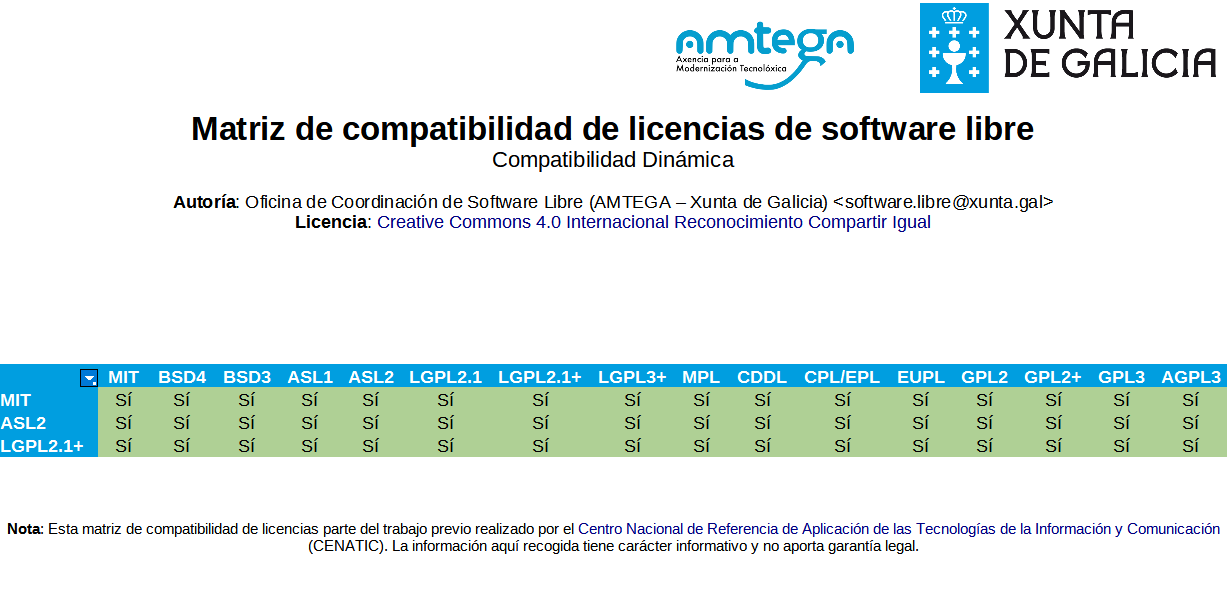
\includegraphics[width=\textwidth]{imagenes/MatrizCompatibilidadDinamica.png}
		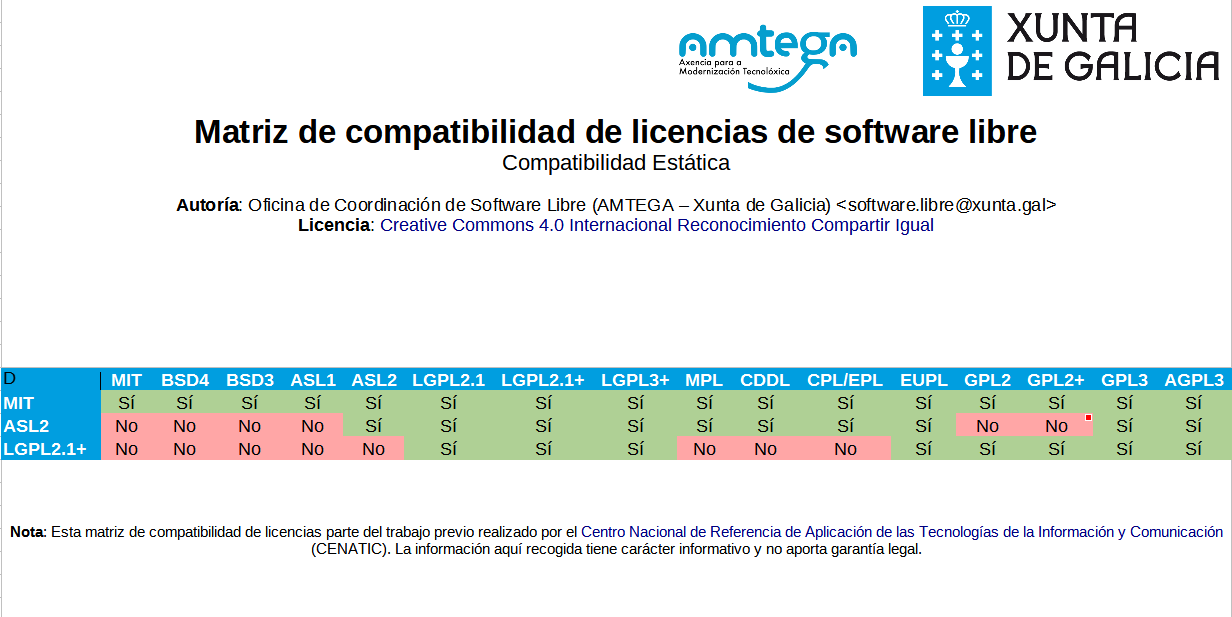
\includegraphics[width=\textwidth]{imagenes/MatrizCompatibilidadEstatica.png}
		\caption{Matriz de compatibilidad de licencias de Software Libre con respecto a licencias Apache 2.0 (ASL2), LGPL 2.1 o superior (LGPL2.1+), y MIT. Matriz extraída de \cite{matriz-licencias}.}
		\label{fig:matrices-comp}
	\end{figure}
\end{center}

A raíz de observar las matrices en la figura \ref{fig:matrices-comp} , tanto la dinámica como la estática, nos quedaríamos con el siguiente listado de candidatos, los cuales listamos anteriormente en la sección \ref{gpl-license-types}:
\begin{itemize}
	\item Lesser GNU Public License 2.1 (con posibilidad de permitir actualizarse a versiones posteriores)
	\item Lesser GNU Public License 3 (con posibilidad de permitir actualizarse a versiones posteriores)
	\item European Union Public License
	\item GNU Public License 3
	\item Affero GNU Public License 3
\end{itemize}

Teniendo en cuenta que las posibilidades de Arcadia se pueden extender a la red gracias a las acciones de Rasa y su posible extensión a un servicio cliente-servidor donde la fuente de conocimiento residiera en un ordenador remoto y el resto de la implementación se quedaría del lado de nuestro ordenador, se opta finalmente por aplicar una licencia AGPL3, la cual se añade al repositorio junto al resto de la documentación.

\begin{table}[H]
	\centering
	\begin{tabularx}{\textwidth}{|>{\columncolor{mintgreen}}c>{\columncolor{mintgreen}}X|}
		\hline
		
\includegraphics[width=30pt]{imagenes/Tarea_completada.png} & Con ello, cumplimos los Objetivos \textbf{O-IA 6.} (Analizar las distintas licencias que se ofrecen y las compatibilidades entre éstas para elegir la idónea para la aplicación resultante.) \\
		\hline
	\end{tabularx}
\end{table}

\subsection{Otros desarrollos que no se han podido completar}
\label{sect:unfinished-dev}
Aparte de lo que se ha realizado para resolver los hitos del proyecto, se han intentado hacer algunas mejoras para facilitar el desarrollo o introducir nuevas funcionalidades, pero han quedado sin éxito tras buscar e investigar sin pdoer conseguir hacer arreglos. Pasamos a listar algunos de ellos:
\begin{itemize}
	\item \textbf{Docker para desarrollo:} Se ha intentado desarrollar un sistema de dos contenedores que hagan ejecutar una instancia de Rasa y otra de nuestro asistente, conectados por una red entre ambos contenedores, con el objetivo de simplificar la ejecución. Al intentar realizarlo, nos hemos encontrado con que al usar las imágenes oficiales del sistema de Chatbot, nos da un error de permisos que no tiene documentada la solución. Tras intentar hacer cambios para que lo aceptara sin éxito, se ha optado por desistir.
	\item \textbf{Segundo hilo para algunas ejecuciones:} Hay cuestiones que precisarían una tarea que se ejecute a la vez que nuestro hilo principal, como puede ser escuchar la radio. Sin embargo, en este momento no se ha conseguido ejecutar un nuevo hilo para estas cuestiones. Se tratará de realizar en un posterior trabajo, permitiendo así la concurrencia y/o paralelismo de las tareas que influyen en Arcadia.
	\item \textbf{Versión para Raspberry Pi}: Si bien sería una buena idea, ya que se podría tener una versión compacta como un prototipo del tamaño de un aparato similar a los competidores con Alexa \cite{alexa} y Echo \cite{echo}, debido a que los contenedores de Docker no están listos, se ha optado por no hacer desarrollos enfocados en la arquitectura ARM que usa esta placa de desarrollo.
\end{itemize}

